\documentclass[a4paper, 12pt]{article}
\usepackage[top=1.5cm, bottom=2.2cm, left=2cm, right=2cm]{geometry}
\usepackage[utf8]{inputenc}
\usepackage{graphicx, caption}
\usepackage{float}
\usepackage{amsmath, amsfonts, amssymb, esint}
\usepackage{hyperref}
\usepackage{multicol}
\usepackage{color}
\usepackage{wallpaper}
\usepackage{array}

\CenterWallPaper{1}{./img/background.png}

\hypersetup{
    colorlinks=true,
    linkcolor=blue,
    filecolor=magenta,      
    urlcolor=cyan,
}

\newcolumntype{M}[1]{>{\centering\arraybackslash}m{#1}}

\definecolor{red}{rgb}{1,0,0}
\newcommand{\red}[1]{\textcolor{red}{#1}}

\begin{document}
    \begin{figure}
        \centering
        \href{https://ligaolimpicadeastronomia.com.br/}{
\includegraphics[scale=0.6]{./img/logos.png}}
    \end{figure}
    \begin{center}
        \begin{large}
            \textbf{Simulado 2 -- Intensivão para a OBA}
            \linebreak \red{Gabarito}
        \end{large}
        \end{center}
    \begin{flushright}
        Material elaborado por \textbf{Giulia Nóbrega} e \textbf{Iago Mendes}.
    \end{flushright}
    \red{Observação: \begin{itemize}
        \item As alternativas das perguntas deste gabarito não estão na mesma ordem do simulado.
    \end{itemize}}

    \section*{Questões de Astronomia}
        \begin{flushleft} \begin{itemize}
            \item \textbf{Questão 1) (1 ponto)} A imagem abaixo traz 2 constelações muito famosas. A partir da imagem, responda o que se pede:
                \begin{figure}[H]
                    \centering
                    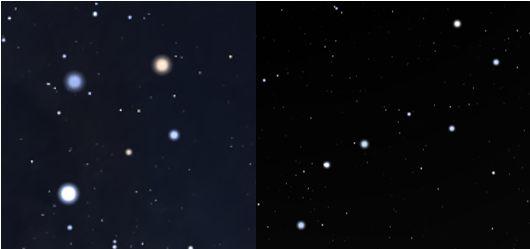
\includegraphics[scale=0.5]{./img/1.png}
                \end{figure}
                \begin{itemize}
                    \item \textbf{Pergunta 1a) (1 ponto) (0,5 ponto cada acerto)} Identifique quais são as constelações na imagem.
                    \begin{center} \begin{tabular}
                    {
                        |M{0.20\textwidth}|M{0.10\textwidth}|M{0.10\textwidth}|M{0.10\textwidth}|M{0.10\textwidth}|
                    }
                        \hline
                        $\quad$ & Centauro & Cruzeiro do Sul & Cisne & Ursa Maior \\ \hline
                        Constelação da esquerda & $\quad$ & \red{X} & $\quad$ & $\quad$ \\ \hline
                        Constelação da direita & $\quad$ & $\quad$ & $\quad$ & \red{X} \\ \hline
                    \end{tabular} \end{center}
                \end{itemize}
            
            \item \textbf{Questão 2) (1 ponto)} Abaixo temos descrições de diversos corpos celestes. Identifique-os:
                \begin{itemize}
                    \item \textbf{Pergunta 2a) (0,25 ponto)} Este corpo constantemente se afasta da Terra. Possui sempre a mesma face voltada para a Terra, ou seja, é bloqueado por marés.
                        \begin{itemize}
                            \item[$(\red{X})$] Lua
                            \item[$(\quad)$] Sol
                            \item[$(\quad)$] Vênus
                            \item[$(\quad)$] Marte
                        \end{itemize}
                    \item \textbf{Pergunta 2b) (0,25 ponto)} Orbita um planeta que possui apenas dois satélites naturais, sendo sua órbita a de menor raio. Com o passar do tempo se aproxima cada vez mais de seu planeta, o que indica que futuramente será despedaçado devido à força gravitacional exercida pelo corpo maior.
                        \begin{itemize}
                            \item[$(\red{X})$] Fobos
                            \item[$(\quad)$] Deimos
                            \item[$(\quad)$] Ceres
                            \item[$(\quad)$] Lua
                        \end{itemize}
                    \item \textbf{Pergunta 3c) (0,5 ponto)} É azulado e possui anéis. Demora aproximadamente 84 anos para completar sua translação. Possui 27 satélites naturais, sendo os principais Miranda, Ariel, Umbriel, Titânia e Oberon. É o menos massivo dos planetas gigantes.
                        \begin{itemize}
                            \item[$(\red{X})$] Urano
                            \item[$(\quad)$] Júpiter
                            \item[$(\quad)$] Saturno
                            \item[$(\quad)$] Netuno
                        \end{itemize}
                \end{itemize}

            \item \textbf{Questão 3) (1 ponto)} Na astronomia muitas vezes é útil estimar a altura de um objeto celeste. Como trabalhamos com corpos muito distantes de nós, a altura que medimos não é um comprimento, e sim um ângulo. Um dos objetos mais famosos utilizados para auxiliar esse cálculo é o sextante, que inclusive dá nome a uma constelação do hemisfério sul. Um aluno da OBA decide tentar fazer o mesmo, porém como não tem um sextante resolve improvisar. Ele finca uma vara de madeira de $1 \, m$ no chão e percebe que a sombra do objeto possui $1,2 \, m$. \linebreak \linebreak Dados: \linebreak $\tan(30^{\circ}) \approx 0,58$ \linebreak $\tan(60^{\circ}) \approx 1,73$ \linebreak \linebreak Dica: \linebreak Lembre-se que para $x$ entre $0^{\circ}$ e $90^{\circ}$ a função $\tan(x)$ é estritamente crescente.
                \begin{itemize}
                    \item \textbf{Pergunta 3) (1 ponto)} Qual é aproximadamente a altura do Sol?
                        \red{\begin{itemize}
                            \item Chamando a altura de Sol de $h$ e usando o cenário descrito, podemos calcular o $\tan h$:
                                \begin{equation*}
                                    \tan h = \frac{1}{1,2} \approx 0,83
                                \end{equation*}
                            \item Usando os valores das tangentes de $30^{\circ}$ e $60^{\circ}$ -- e lembrando que $\tan (40^{\circ}) = 1$ --, deduzimos que $30^{\circ} \leq h \leq 45^{\circ}$. Portanto, a única alternativa válida é $40^{\circ}$
                        \end{itemize}}
                        \begin{itemize}
                            \item[$(\quad)$] $10^{\circ}$
                            \item[$(\red{X})$] $40^{\circ}$
                            \item[$(\quad)$] $60^{\circ}$
                            \item[$(\quad)$] $80^{\circ}$
                        \end{itemize}
                \end{itemize}
        \end{itemize} \end{flushleft}
    \section*{Questões de Astronáutica}
    \section*{Questões avançadas}
\end{document}